\documentclass[UTF8,openany,AutoFakeBold,AutoFakeSlant,cs4size]{ctexbook}
%openany 使一章可以从偶数页开始,因为说明中每一章并没有只能从奇数页开始,虽然这是常理
%AutoFakeBold 和 AutoFakeSlant 因为 CJK 里没有真正的加粗和倾斜,如果额外字体则效果更好
%cs4size 因为要求主题是小四号字

%\usepackage[a4paper,left=5cm,right=0cm,top=2.5cm,bottom=2.5cm,twoside]{geometry}
\usepackage[a4paper,left=2.5cm,right=2cm,top=2.5cm,bottom=2.5cm,twoside]{geometry}

\usepackage{amsmath}
\usepackage{bm}
\usepackage{amsfonts}
\usepackage{enumerate}
\usepackage{fancyhdr}

\usepackage{cite}
\newcommand{\upcite}[1]{\textsuperscript{\cite{#1}}} %引用在右上角

\usepackage{multirow,booktabs,makecell}
\usepackage{graphicx}
\usepackage[font=small,labelsep=space]{caption} %五号,宋体/Time new roman
%\renewcommand{\thetable}{\arabic{table}} %表格和图片编号不分章节,直接1,2,3 ...
%\renewcommand{\thefigure}{\arabic{figure}}
\renewcommand{\theequation}{\arabic{chapter}.\arabic{equation}} %公式标签 章.公式(均为阿拉伯数字)

\usepackage{tocloft} %自定义目录,说明中没有明确规定,和WORD自动生成目录格式一致

%“全文目录”四个字的格式
\renewcommand\cftbeforetoctitleskip{0pt}
\renewcommand\cftaftertoctitleskip{0pt}
\renewcommand\cfttoctitlefont{\bfseries\heiti\zihao{2}}

\renewcommand\cftchapfont{\heiti\normalsize} %黑体小四
\renewcommand\cftchapdotsep{\cftdotsep} %有点连到页码,点间距不确定,待改
\renewcommand\cftchappagefont{\songti\normalsize} %宋体小四页码
\renewcommand\cftbeforechapskip{0pt}

%1. 第一级 五号宋体,缩进两个字符,页码一致
\renewcommand\cftsecfont{\songti\small}
\renewcommand\cftsecpagefont{\songti\small}
\renewcommand\cftsecaftersnum{.} %一级目录号后加点
\renewcommand\cftsecindent{2em}
\renewcommand\cftbeforesecskip{0pt}

%1.1 第二级 五号宋体,缩进四个字符,页码一致
\renewcommand\cftsubsecfont{\songti\small}
\renewcommand\cftsubsecpagefont{\songti\small}
\renewcommand\cftsubsecindent{4em}
\renewcommand\cftbeforesubsecskip{0pt}

%1.1.1 第二级 五号宋体,缩进四个字符,页码一致
\renewcommand\cftsubsubsecfont{\songti\small}
\renewcommand\cftsubsubsecpagefont{\songti\small}
\renewcommand\cftsubsubsecindent{4em}
\renewcommand\cftbeforesubsubsecskip{0pt}

\usepackage{titlesec}%自定义章节标题
\CTEXsetup[format={\center\heiti\zihao{3}},beforeskip=0pt]{chapter}
%第一章  绪论(二号、黑体) beforeskip为上方垂直距离看起来还比说明偏大,待改

\setcounter{tocdepth}{3}
\setcounter{secnumdepth}{3}
%使目录中有三级标题,即subsubsection

%\renewcommand\thesection{\arabic{section}} % 使得不显示章名你妈呀
\titleformat{\section}
{\raggedright\zihao{3}\songti}
{\thesection\quad}
{0pt}
{}%1. 第一级(三号、宋体/Time new roman、加粗你妈)

\titleformat{\subsection}
{\raggedright\zihao{4}\songti}
{\thesubsection\quad}
{0pt}
{}%1.1 第二级(四号,宋体/Time new roman,加粗你妈)

\titleformat{\subsubsection}
{\raggedright\zihao{-4}\songti}
{\thesubsubsection\quad}
{0pt}
{}%1.1.1 第三级(小四,宋体/Time new roman,加粗你妈)

% 封面依赖的宏包
\usepackage{xcoffins} % 用于设计封面格式
\usepackage{xcolor}
\usepackage{soul} % 用于设置下划线宽度
\setul{}{2pt}
\setmainfont{Times New Roman} % Times New Roman 作为默认英文字体

% 评阅表依赖的宏包
\usepackage{float}
\usepackage{array}
\usepackage{makecell}


% your includes here
\usepackage{colortbl}
\usepackage{xspace}
\newcommand{\chineseTitleA}{基于深度学习的}
\newcommand{\chineseTitleB}{壹壹肆伍壹肆壹玖壹玖捌壹零}
\newcommand{\englishTitleA}{Beyond P=NP: One One Four}
\newcommand{\englishTitleB}{Five One Four is All You Need}
\newcommand{\name}{唐可可}
\newcommand{\studentID}{1800099999}
\newcommand{\school}{信息科学技术学院(本科生学院)}
\newcommand{\major}{计算机科学与技术}
\newcommand{\advisor}{田中仁}
\newcommand{\advisorAffiliation}{偶像同好会}
\newcommand{\advisorTitle}{永远的神}

% 打印前请去除main.tex中documentclass的screen选项,以应用奇偶页不对称(装订线5mm)的排版效果
% 去除后将不再显示此内容
\newcommand{\buildInfo}{\center\colorbox{yellow}{build \today{} at \DTMcurrenttime{}, screen mode}}
% 或者可以这样保留screen选项并不显示此内容:
%\renewcommand{\buildInfo}{}

\newcommand{\advisorComment}{
% ↓ adjust total height below
\begin{minipage}[t][15cm][t]{\linewidth-2em}

\begin{center}
    \kaishu{(包含对论文的性质、难度、分量、综合训练等是否符合培养目标的目的等评价)}
\end{center}

\setlength{\parindent}{2em}

% https://zh.moegirl.org.cn/NEO_SKY,_NEO_MAP!

今日湛蓝的天空已不同于昨日,
明天的蓝天又会与今日不甚相同。
在你的眼中,也在我的眼中……
啊啊,已经无法用言语表述。

这种时候 如果你在我身边,
会松一口气呢。
所以,
所以明天也要抬头仰望,
在这里,和你一起。
自由地描绘这崭新的地图吧,
NEO MAP!

虽然还不知道要去往何方,
但那有趣的未来早已等待。
能有你与我一同欢笑,就会很快乐,
今天也感谢有你。

现在,就从现在开始,展开各自的地图。
轻松地飞奔而出吧。
梦想着,憧憬着,还想再次见证梦想,
想看到,真想看到呢。

NEO SKY, NEO MAP!
NEO SKY, NEO MAP!

\end{minipage}
}

\newcommand{\reviewDate}{\makebox[4em][c]{1919}年\makebox[2em][c]{8}月\makebox[2em][c]{10}日}
\newcommand{\honorDate}{\makebox[4em][c]{1145}年\makebox[2em][c]{1}月\makebox[2em][c]{4}日}


\title{}
\author{}
\date{}

\begin{document}

% 插入封面
% 声明需要的Coffin
\NewCoffin \result
\NewCoffin \topBox
\NewCoffin \pkuLogo
\NewCoffin \headingText
\NewCoffin \titleText
\NewCoffin \chineseTitleTextA
\NewCoffin \chineseTitleTextB
\NewCoffin \englishTitleTextA
\NewCoffin \englishTitleTextB
\NewCoffin \nameText
\NewCoffin \studentIDText
\NewCoffin \schoolText
\NewCoffin \majorText
\NewCoffin \advisorText
\NewCoffin \dateText

% 各个Coffin的内容
\SetHorizontalCoffin \result {}
\SetHorizontalCoffin \topBox {\color{white} \rule{210mm}{41mm}}
\SetHorizontalCoffin \pkuLogo {
\includegraphics[width=83.9mm]{head/pku_logo}}
\SetVerticalCoffin \headingText{160mm}{\center\heiti\fontsize{36}{36}\textcolor{black}{本科生毕业论文}}
\SetVerticalCoffin \titleText{25.4mm}{\songti\zihao{3}{题目:}}
\SetVerticalCoffin \chineseTitleTextA{110mm}{\bfseries\heiti\zihao{2}\underline{\makebox[114mm][l]{\hfill \chineseTitleA \hfill}}}
\SetVerticalCoffin \chineseTitleTextB{110mm}{\bfseries\heiti\zihao{2}\underline{\makebox[114mm][l]{\hfill \chineseTitleB \hfill}}}
\SetVerticalCoffin \englishTitleTextA{110mm}{\bfseries\heiti\zihao{2}\underline{\makebox[114mm][l]{\hfill \englishTitleA \hfill}}}
\SetVerticalCoffin \englishTitleTextB{110mm}{\bfseries\heiti\zihao{2}\underline{\makebox[114mm][l]{\hfill \englishTitleB \hfill}}}
\SetVerticalCoffin \nameText{114mm}{\center\heiti\fontsize{16}{16}\textcolor{black}{姓\qquad\ \ \ 名:\underline{\makebox[86mm][c]{\kaiti{\name}}}}}
\SetVerticalCoffin \studentIDText{114mm}{\center\heiti\fontsize{16}{16}\textcolor{black}{学\qquad\ \ \ 号:\underline{\makebox[86mm][c]{\kaiti\zihao{3}{\studentID}}}}}
\SetVerticalCoffin \schoolText{114mm}{\center\heiti\fontsize{16}{16}\textcolor{black}{院\qquad\ \ \ 系:\underline{\makebox[86mm][c]{\kaiti{\school}}}}}
%\SetVerticalCoffin \majorText{104mm}{\center\songti\fontsize{16}{16}\textcolor{black}{本科专业:\underline{\makebox[76mm][c]{\kaiti{\major}}}}}
\SetVerticalCoffin \majorText{114mm}{\center\heiti\fontsize{16}{16}\textcolor{black}{专\qquad\ \ \ 业:\underline{\makebox[86mm][c]{\kaiti{\major}}}}}
\SetVerticalCoffin \advisorText{114mm}{\center\heiti\fontsize{16}{16}\textcolor{black}{导师姓名:\underline{\makebox[86mm][c]{\kaiti{\advisor}}}}}
\SetVerticalCoffin \dateText{114mm}{\center\heiti\fontsize{18}{18}\textcolor{black}二\hspace{-2pt}\raisebox{-2pt}{\huge 〇}\hspace{-2pt}二二年六月}


% 指定各个Coffin相对位置关系
\JoinCoffins \result \topBox
\JoinCoffins \result[\topBox-hc, \topBox-b] \pkuLogo[hc, b](0mm, -10.6mm)
\JoinCoffins \result[\topBox-hc, \topBox-b] \headingText[hc, b](0mm, -28.8mm)
\JoinCoffins \result[\headingText-hc, \headingText-b] \titleText[l, t](-77.25mm, -16mm)
\JoinCoffins \result[\headingText-hc, \headingText-b] \chineseTitleTextA[l, t](-62.85mm, -14.85mm)
\JoinCoffins \result[\headingText-hc, \headingText-b] \chineseTitleTextB[l, t](-62.85mm, -26.85mm)
\JoinCoffins \result[\headingText-hc, \headingText-b] \englishTitleTextA[l, t](-62.85mm, -38.85mm)
\JoinCoffins \result[\headingText-hc, \headingText-b] \englishTitleTextB[l, t](-62.85mm, -50.85mm)
\JoinCoffins \result[\headingText-hc, \headingText-b] \nameText[hc, t](0mm, -90mm)
\JoinCoffins \result[\nameText-hc, \nameText-b] \studentIDText[hc, t](0mm, 0mm)
\JoinCoffins \result[\studentIDText-hc, \studentIDText-b] \schoolText[hc, t](0mm, 0mm)
\JoinCoffins \result[\schoolText-hc, \schoolText-b] \majorText[hc, t](0mm, 0mm)
\JoinCoffins \result[\majorText-hc, \majorText-b] \advisorText[hc, t](0mm, 0mm)
\JoinCoffins \result[\advisorText-hc, \advisorText-b] \dateText[hc, t](0mm, -40mm)


% 输出封面
\thispagestyle{empty}
\newgeometry{left=.25cm, bottom=0mm, top=0mm, right=0mm}
\noindent\TypesetCoffin \result
\restoregeometry
\clearpage

% 插入导师评阅表
\thispagestyle{empty}
\renewcommand\arraystretch{1.2}

\begin{center}
{\songti\zihao{3}{北京大学本科毕业论文导师评阅表}}
\end{center}

\begin{table}[H]
	\centering
    \begin{tabular}{|rrrrrr|}
    \hline
    \multicolumn{1}{|p{4em}|}{学生姓名} & \multicolumn{1}{p{3em}|}{\name} & \multicolumn{1}{p{5em}|}{学生学号} & \multicolumn{1}{p{6em}|}{\studentID} & \multicolumn{1}{p{6em}|}{论文成绩} &  \multicolumn{1}{l|}{\paperGrade}\\
    \hline
    \multicolumn{1}{|l|}{学院(系)} & \multicolumn{3}{l|}{\school} & \multicolumn{1}{l|}{学生所在专业} & \multicolumn{1}{l|}{\major} \\
    \hline
    \multicolumn{1}{|l|}{导师姓名} & \multicolumn{1}{l|}{\advisor} & \multicolumn{1}{l|}{\makecell{导师单位/\\所在研究所}} & \multicolumn{1}{l|}{\advisorAffiliation} & \multicolumn{1}{l|}{导师职称} & \multicolumn{1}{l|}{\advisorTitle} \\
    \hline
    \multicolumn{2}{|c|}{\makecell{论文题目\\(中、英文)}} & \multicolumn{4}{c|}{\makecell{\chineseTitleA{}\chineseTitleB{}\\ \englishTitleA{} \englishTitleB{}}} \\
    \hline
    \multicolumn{6}{|c|}{导师评语} \\
    \multicolumn{6}{|c|}{\advisorComment{}} \\
    \multicolumn{6}{|r|}{
        导师签名:
        \begin{tikzpicture}[overlay]
            \node[anchor=south west,yshift=-1em] at (0,0) {
                
\includegraphics[height=2em]{figures/sign-advisor}
            };
        \end{tikzpicture}
        \hspace{8em} 
    } \\
    \multicolumn{6}{|c|}{} \\
    \multicolumn{6}{|r|}{\reviewDate{}\hspace{2em} } \\
    \multicolumn{6}{|c|}{} \\
    \hline
    \end{tabular}
\end{table}

\renewcommand\arraystretch{1}
\clearpage

\linespread{1.5}\selectfont
\chapter*{版权声明}
% 本页不计页码
\thispagestyle{empty}
% 本页无页眉和页脚
任何收存和保管本论文各种版本的单位和个人,未经本论文作者同意,不得将本论文转借他人,亦不得随意复制、抄录、拍照或以任何方式传播。否则,引起有碍作者著作权之问题,将可能承担法律责任。
\clearpage

%版权声明后空白你妈一页,使得摘要从奇数页开始。
%\quad
% 本页不计页码
%\thispagestyle{empty}
% 本页无页眉和页脚
%\clearpage

\normalsize
\linespread{1.5}\selectfont
%小四号,宋体/Time new roman,1.5倍行距
\chapter*{摘要}

壹壹肆伍壹肆是一个重大问题。

本文壹玖壹玖捌壹零。

\bigskip
\bigskip

关键词: 壹壹肆,伍壹肆
\thispagestyle{empty}
\clearpage

\small
\linespread{1.5}\selectfont
%5号,Time new roman,1.5倍行距
\chapter*{\bfseries ABSTRACT}
\noindent

One one four five one four.

Money is all you need.

\bigskip
\bigskip

KEY WORDS: Foo, Bar
\thispagestyle{empty}
\clearpage

\chapter*{目录}
\renewcommand{\contentsname}{}
\tableofcontents
\thispagestyle{empty}
%\addcontentsline{toc}{chapter}{全文目录}
\clearpage

\normalsize
\linespread{1.5}\selectfont
%正文,小四号,中文宋体,英文Time new roman,1.5倍行距
\fancypagestyle{plain} %因为latex默认每章第一页是plain所以需要重置一下plain和说明统一
{
	\fancyhf{}
    \chead{\chineseTitleA\chineseTitleB}
	\cfoot{第\thepage{}页}
	\renewcommand{\headrulewidth}{0.7pt}
	\renewcommand{\footrulewidth}{0pt}
}

%默认的风格是fancy,设置于下,用于每章非第一页
\fancyhf{}
\chead{\chineseTitleA\chineseTitleB}
\cfoot{第\thepage{}页}
\renewcommand{\headrulewidth}{0.7pt}
\renewcommand{\footrulewidth}{0pt}

\setcounter{page}{1}

\chapter{引言}

\section{哼哼}
\subsection{啊啊啊}
\subsubsection{啊啊啊啊啊}

引用如\cite{Wilt2010beamsearch},引用表如表\ref{tab:input_output_r},引用图如图\ref{fig:sample}。

哈哈哈\footnote{嗯嗯嗯}。

\begin{table}[h]
    \small
    \centering
    \caption{不同频率下的输入和输出阻抗}
    \label{tab:input_output_r}
    \begin{tabular}{cccc}
        \toprule %不确定说明中三条线的粗细,待改
        频率(Hz) & 1 & 10k & 1M \\
        \midrule
        输入电阻($\Omega/^\circ$) & 339.719k/-87.84 & 5.6707k/-9.827 & 351.188/-72.377\\
        输出电阻($\Omega/^\circ$) & 338.638k/-89.663 & 1.9866k/-1.1228 & 1.9189k/-14.801 \\
        \bottomrule
    \end{tabular}
\end{table}

\begin{figure}[h]
    \centering
    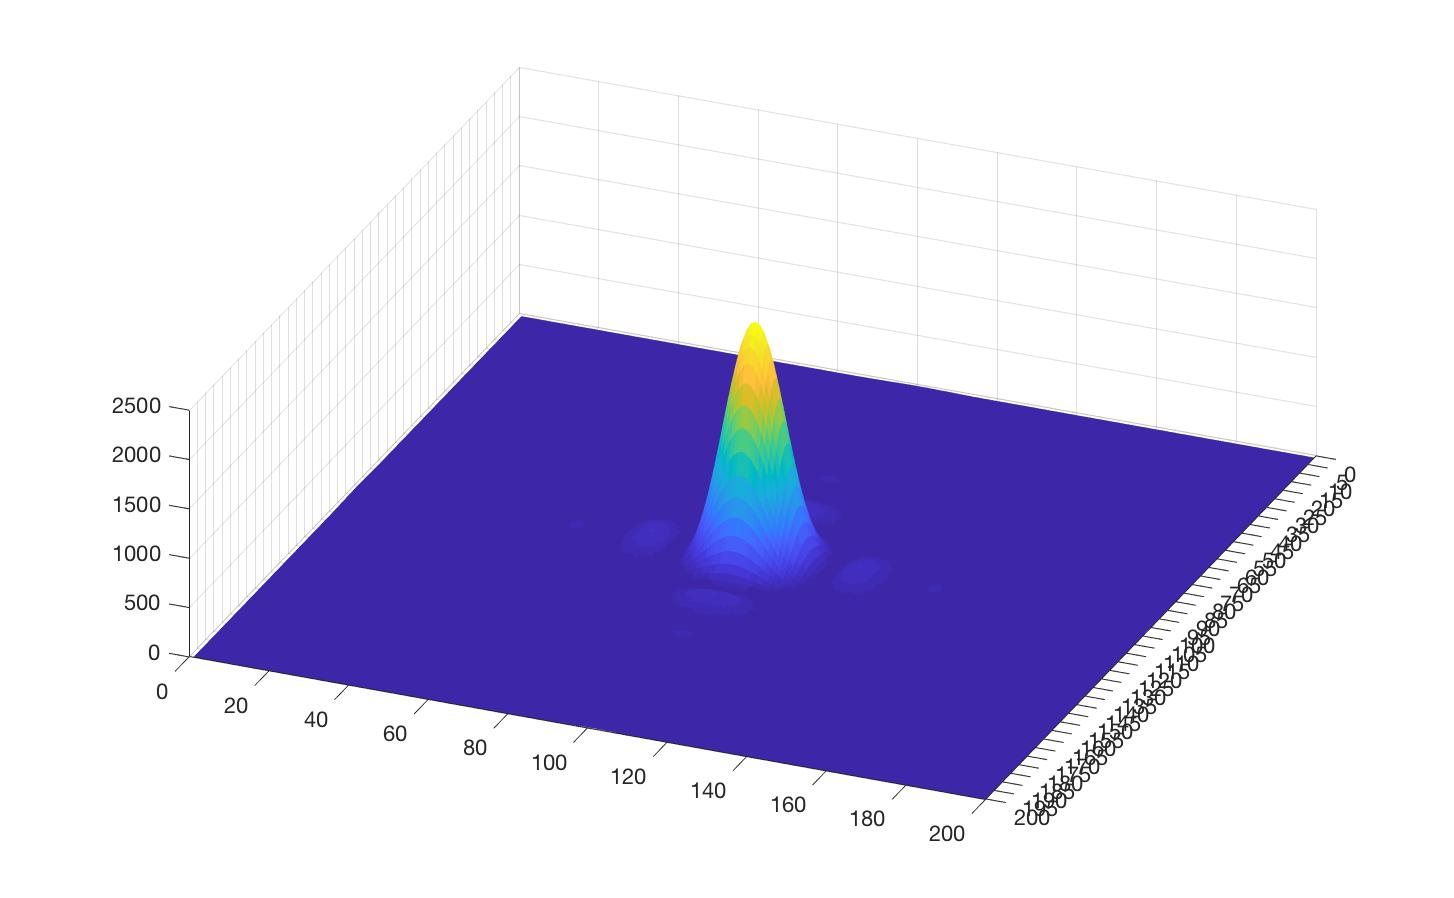
\includegraphics[width=12cm]{figures/Sample.jpg}
    \caption{示例图片}
    \label{fig:sample}
\end{figure}

\chapter{动机}

教练我想学Java~\upcite{jls8}。
\chapter{结论}

嘿嘿唐可可嘿嘿。

\small
\linespread{1}\selectfont
%正文,五号,中文宋体,英文Time new roman,1倍行距
\addcontentsline{toc}{chapter}{参考文献}
\bibliographystyle{unsrt}
\bibliography{bib/base}

\clearpage

% \linespread{1}\selectfont
% \normalsize
% %小四号,中文宋体,英文Time new roman,1倍行距
% \chapter*{本科期间的主要工作和成果}

% \noindent 本科期间参加的主要科研项目

% \noindent 本研基金
% \begin{enumerate}
% 	\item 基金名称. 基金类型. 指导老师. 基金支持年限
% \end{enumerate}

% \noindent 各种科研项目
% \begin{enumerate}
% 	\item 项目名称. 项目类型
% \end{enumerate}

% \addcontentsline{toc}{chapter}{本科期间的主要工作和成果}
% \fancypagestyle{plain}
% {
% 	\fancyhf{}
% 	\fancyhead[RE,RO]{本科期间的主要工作和成果}
% 	\fancyhead[LE,LO]{北京大学本科生毕业论文}
% 	\fancyfoot[CO,CE]{~\thepage~}
% 	\renewcommand{\headrulewidth}{0.7pt}
% 	\renewcommand{\footrulewidth}{0pt}
% }
% \fancyhf{}
% \fancyhead[RE,RO]{本科期间的主要工作和成果}
% \fancyhead[LE,LO]{北京大学本科生毕业论文}
% \fancyfoot[CO,CE]{~\thepage~}
% \renewcommand{\headrulewidth}{0.7pt}
% \renewcommand{\footrulewidth}{0pt}
% \clearpage

\linespread{1.5}\selectfont
\normalsize
%正文,小四号,中文宋体,英文Time new roman,1.5倍行距
\chapter*{致谢}
\addcontentsline{toc}{chapter}{致谢}

谢谢你。

因为有你。

温暖了四季。
\clearpage

\chapter*{北京大学学位论文原创性声明和使用授权说明}
\addcontentsline{toc}{chapter}{北京大学学位论文原创性声明和使用授权说明}
\begin{center}
    \zihao{4}\textbf{原创性声明}
\end{center}

本人郑重声明:所呈交的学位论文,是本人在导师的指导下,独立进行研究工作所取得的成果。除文中已经注明引用的内容外,本论文不含任何其他个人或集体已经发表或撰写过的作品或成果。对本文的研究做出重要贡献的个人和集体,均已在文中以明确方式标明。本声明的法律结果由本人承担。

\bigskip

\begin{flushright}
    论文作者签名:\hspace{10em} \\
    \vspace{1em}
    日期:\hspace{4em}年\hspace{2em}月\hspace{2em}日
\end{flushright}

\bigskip
\bigskip

\begin{center}
    \zihao{4}\textbf{学位论文使用授权说明}
\end{center}

本人完全了解北京大学关于收集、保存、使用学位论文的规定,即:
\begin{itemize}
    \item 按照学校要求提交学位论文的印刷本和电子版本;
    \item 学校有权保存学位论文的印刷本和电子版,并提供目录检索与阅览服务,在校园网上提供服务;
    \item 学校可以采用影印、缩印、数字化或其它复制手段保存论文;
\end{itemize}

\bigskip

\begin{flushright}
    论文作者签名:\hspace{5em} 导师签名:\hspace{5em} \\
    \vspace{1em}
    日期:\hspace{4em}年\hspace{2em}月\hspace{2em}日\hspace{5em} 
\end{flushright}
\thispagestyle{empty}

\end{document}
